\documentclass{../../ece-report}

\usepackage{subcaption}
\usepackage{multirow}


\memostudent{Ty Davis}
\memotitle{Lab 9 - BJT DC Biasing}
\memocourse{ECE 3110}
\memodate{\today}

\begin{document}

\maketitle

\section*{Introduction}

In this lab we are analyzing the DC operating points
of an NPN-type BJT. There are three modes of operation
for a BJT, namely \emph{active}, \emph{saturation},
and \emph{cutoff}. We are going to analyze the BJT in
both the \emph{active} and \emph{saturation} regions
of operation.

Fig.~\ref{fig:circuit} shows our circuit. For each mode
of operation we will select different resistor values
in order to bias the circuit.

\begin{figure}[h!]
  \centering
  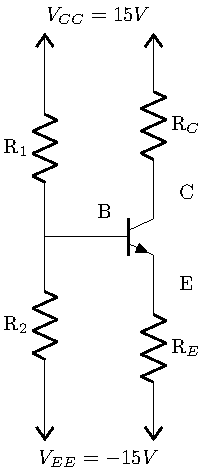
\includegraphics{../circuit/circuit.pdf}
  \caption{The circuit we use in the lab.}
  \label{fig:circuit}
\end{figure}

\section*{Analysis}

\subsection*{Active Mode Operation}

For active mode operation we are going to design the
circuit such that $I_C = 1$~mA, $V_B = 0$~V, and $V_C
= 5$~V.

We can quickly find $I_B$ because we know that
$\beta$ from the data sheet is $\beta=161.205$.
This means that $I_B = I_C/\beta = 6.203~\si{\uA}$.
Knowing that $I_E = I_C + I_B$, we get $I_E = 1.006203$~mA.

With these values we can find $R_C = \frac{15 - 5}{1~\si{\mA}}
= 10~\si{\kohm}$. Using the constant drop model, we
can assume that $V_E = V_B - 0.7~\si{\V} = -0.7~\si{\V}$.
This leads us to $R_E = \frac{-0.7 - (-15)}{1.006203~\si{\mA}}
= 14.371~\si{\kohm}$.

For the remaining two resistors, the function is not
fully specified, but we know that $V_B = 0~\si{\V}$,
and the current through $R_1$ is equal to the current
through $R_2$ and the current $I_B$. As such, we can
do some brief nodal analysis to find:

\[
  \frac{V_{CC} - 0}{R_1} + \frac{0 - V_{EE}}{R_2} + I_B = 0
\]

Rearranging this to solve for $R_1$ in terms of $R_2$ we find this equation:

\[
  R_1 = V_{CC} \cdot \Big( \frac{1}{-I_B - V_{EE} / R_2} \Big)
\]

That expression allowed us to choose some $R_2$ and determine
a necessary $R_1$. We chose the value $R_2 = 100~\si{\kohm}$,
and the corresponding $R_1$ is found to be $R_1 = 96.028~\si{\kohm}$.

\section*{Saturation Mode Operation}

The Saturation Mode operation is even more straightforward.
We are going to design the circuit such that $I_C =
1~\si{\mA}$, $I_E = 0.2~\si{\mA}$, $V_C = 2~\si{\V}$,
and $V_{CE}=0.2~\si{\V}$. 

Knowing $I_C$ and $I_B$ means that we can find $I_E
= 200~\si{\uA}$. Also, we find that $V_E = 1.8~\si{\V}$ 
because $V_{CE} = 0.2~\si{\V}$.

With values for $V_C$ and $V_E$ we can find that $R_C
= 13~\si{\kohm}$ and $R_E = 14~\si{\kohm}$. 

The same method for calculating $R_1$ and $R_2$ applies
in this circuit as well, so we can select $R_2 = 100~\si{\kohm}$
and find that $R_1 = 33.333~\si{\kohm}$.

The $\beta_\textnormal{forced}$ that we found is $\frac{1~\si\mA}{200~\si{\uA}} = 5$.


\section*{Simulation Results}

Building the circuit in Multisim we recorded the following values:


\begin{table}[h!]
  \centering
  \begin{tabular}{c l l}\toprule
      & \textbf{Active Mode} & \textbf{Saturation Mode} \\
    \midrule
    $V_C$     & 5.12~\si{\V}   &  1.92~\si{\V}  \\
    $V_B$     & -40.0~\si{\mV} &  2.54~\si{\V}  \\
    $V_E$     & -0.704~\si{\V} &  1.86~\si{\V}  \\
\midrule
    $V_{BE}$  & 0.66~\si{\V}  &  0.68~\si{\V}   \\
    $V_{CE}$  & 5.82~\si{\V}  &  0.08~\si{\V}   \\
    $I_C$     & 0.988~\si{\mA} &  1.01~\si{\mA}\\
    $I_B$     & 7.02~\si{\uA}  &  198.68~\si{\uA} \\
    $I_E$     & 0.995~\si{\mA} &  1.20~\si{\mA}\\
\bottomrule
\end{tabular}
\caption{Simulation results.}
\label{tab:sim_results}
\end{table}



\section*{Measurement Results}

Building the circuit we found that the our analysis
and simulation in both active mode and saturation mode
operation were very close to the actual performance
of the device. Look at Tables~\ref{tab:active_resistors}
and \ref{tab:sat_resistors} to see the resistor values
that we used.

The $\beta_\textnormal{forced}$ that we calculated is
$\frac{1.012~\si\mA}{205.7~\si\uA} = 4.921$.



\begin{table}[h!]
  \centering
  \begin{tabular}{c l l}\toprule
      & \textbf{Active Mode} & \textbf{Saturation Mode} \\
    \midrule
    $V_C$     & 5.06~\si{\V}   &  1.918~\si{\V}  \\
    $V_B$     & -3.0~\si{\mV}  &  2.546~\si{\V}  \\
    $V_E$     & -0.661~\si{\V} &  1.873~\si{\V}  \\
\midrule
    $V_{BE}$  & 0.658~\si{\V}   & 0.673~\si{\V}   \\
    $V_{CE}$  & 5.721~\si{\V}   & 0.045~\si{\V}   \\
    $I_C$     & 1.00638~\si{\mA} & 1.01215~\si{\mA}\\
    $I_B$     & 5.12 ~\si{\uA}   & 205.68~\si{\uA} \\
    $I_E$     & 1.0115 ~\si{\mA}   & 1.21783~\si{\mA}\\
\bottomrule
\end{tabular}
\caption{Measurement results.}
\label{tab:meas_results}
\end{table}


\begin{table}[h!]
  \centering
  \begin{tabular}{l l l c}\toprule
    \textbf{Calculated Resistor} & \textbf{Equivalent Resistor} & \textbf{Measured Resistor} & \\
    \midrule

10 \si{\kohm} & 10 \si{\kohm} & 9.877 \si{\kohm} & $R_C$ \\
          \midrule
14.371 \si{\kohm}    & 14.347 \si{\kohm}    & 14.176 \si{\kohm}    & $R_E$ \\
          & 15 \si{\kohm}    & 14.82   \si{\kohm}  &       \\
          & 330 \si{\kohm}    & 325.38   \si{\kohm}  &       \\
          \midrule
96.028 \si{\kohm}     & 96.2 \si{\kohm}     & 95.542 \si{\kohm}  & $R_1$ \\
          & 47 \si{\kohm}     & 46.689 \si{\kohm}   &       \\
          & 47 \si{\kohm}     & 46.679 \si{\kohm}   &       \\
          & 2.2 \si{\kohm}    &  2.173 \si{\kohm}   &       \\
\midrule
100 \si{\kohm}     & 100 \si{\kohm}     & 98.75 \si{\kohm}  & $R_2$ \\
\bottomrule
\end{tabular}
\caption{Active Mode Resistors.}
\label{tab:active_resistors}
\end{table}


\begin{table}[h!]
  \centering
  \begin{tabular}{l l l c}\toprule
    \textbf{Calculated Resistor} & \textbf{Equivalent Resistor} & \textbf{Measured Resistor} & \\
    \midrule

13 \si{\kohm} & 13.043 \si{\kohm} & 12.925 \si{\kohm} & $R_C$ \\
          & 15 \si{\kohm}    & 14.86   \si{\kohm}  &       \\
          & 100 \si{\kohm}    & 99.35   \si{\kohm}  &       \\
          \midrule
14 \si{\kohm}    & 14.042 \si{\kohm}    & 13.855 \si{\kohm}    & $R_E$ \\
          & 15 \si{\kohm}    & 14.82   \si{\kohm}  &       \\
          & 220 \si{\kohm}    & 217.68   \si{\kohm}  &       \\
          \midrule
96.028 \si{\kohm}     & 96.2 \si{\kohm}     & 95.542 \si{\kohm}  & $R_1$ \\
          & 47 \si{\kohm}     & 46.689 \si{\kohm}   &       \\
          & 47 \si{\kohm}     & 46.679 \si{\kohm}   &       \\
          & 2.2 \si{\kohm}    &  2.173 \si{\kohm}   &       \\
\midrule
100 \si{\kohm}     & 100 \si{\kohm}     & 98.75 \si{\kohm}  & $R_2$ \\
\bottomrule
\end{tabular}
\caption{Active Mode Resistors.}
\label{tab:sat_resistors}
\end{table}

\end{document}
